\section{Synchronization Design}
The purpose of the synchronization is to maintain a local database on an Android device that can be kept in synchronization with the central database. The idea behind the synchronization is that many different Android devices should be able to access information about the same users. For this to work correctly, the data on different Android devices should be the same, otherwise the concept of a central database that stores all data will be moot. This means that the database on the Android device will include exact copies of relevant data that the central database includes, and as such the two databases must have the same tables. In addition to downloading data from the central database, an Android device will be able to create data itself. This data can then be uploaded to the central database to be kept in synchronization with many different devices.

The application that will synchronize the data between Android devices and the central database will run on the Android devices, and will thus be written in Java.

\subsection{The Application}
The application for synchronization, henceforth known as Puddle, is meant to be a replacement of the OasisLib application from previous years.

\begin{figure}[hptb]
    \begin{center}
    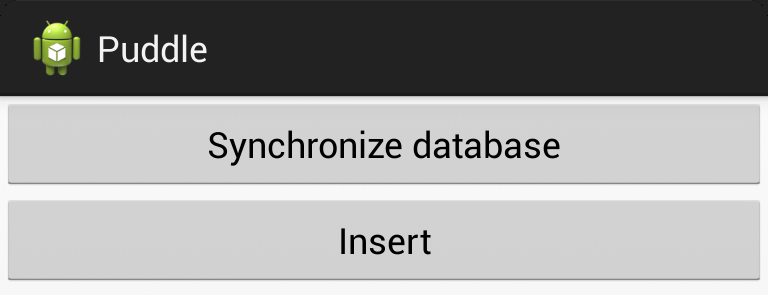
\includegraphics[width=0.8\textwidth]{img/puddle-app.png}
    \caption{Overview of the Puddle Android application.}
    \label{fig:puddle_app}
    \end{center}
\end{figure}

\autoref{fig:puddle_app} shows the Puddle application as it launches on an Android device. Puddle has two buttons, one for synchronizing with the central database, and one for inserting information into the local database. Puddle synchronizes manually with the central database, and needs to be launched manually. To synchronize, press the synchronize button, and Puddle will upload changes made to the local database, and then download from the central database. When the insert button is pressed, it inserts data into the database.

\subsection{Creating a Local Database}
Before it is possible to save to a local database on an Android device, it must first be created. Android only has native support for SQLite to create SQL databases, SQLite is therefore used for the local database in Puddle.
The local database is not created until it is needed. This means that the local database will not be created until the synchronization with the central database is started. The local database is not deleted, however, unless it is actively requested. On subsequent synchronizations there is no need to create the local database again.

\subsection{Uploading and Downloading Changes}
Changes made on an Android device should not be deleted when the two databases are synchronized. To avoid it, the updated data are first uploaded to the central database, before new data from the central database is downloaded to the Android device. This has the unfortunate side effect that if the same data was changed on both the central and local database between synchronizations, one has to take precedence over the other. It was decided that changes made on Android devices will always supersede changes made to the central database.

Before uploading changes made on the Android device, the changes must be found. To find these, a table has been added to the local database that does not exist in the central database. This table contains a timestamp with the time of the most recent synchronization with the central database. An additional attribute is added to all tables in the local database. This attribute also contains a timestamp, but this timestamp is updated when the row is inserted or changed. Every row that has a newer timestamp than the last synchronization is new or has been updated. These will be uploaded to the central database at the next synchronization. If there are no changes, this step will be skipped. Next, the data on the central database is downloaded to the Android device and its database is updated with this. Of course, only data that is newer than the timestamp of the last synchronization and is relevant for users of the device is downloaded.


